\documentclass{beamer}

\usepackage{graphicx}
\usepackage{caption}
\usepackage{subcaption}

\usepackage{algpseudocode}
\usepackage{algorithm}
\usepackage{algorithmicx}


\usetheme{metropolis}           % Use metropolis theme
\title{Whale Optimization Algorithm (WOA) para el problema de clustering con restricciones}
\date{\today}
\author{Yábir García Benchakhtir}
\institute{Universidad de Granada}
\begin{document}
  \maketitle

\section{Descripción del problema}
\begin{frame}{Etapas en la caza}
    Resolvemos el problema del agrupamiento con restricciones

    \begin{itemize}
        \item Partimos de un conjunto de puntos
        \item Una serie de restricciones entre ellos
    \end{itemize}
    \pause
    Nuestro objetivo es agruparlos en conjuntos de manera que haya relación
    entre los elementos de un mismo conjunto minimizando el número de
    restricciones incumplidas.

\end{frame}

\begin{frame}
    Algunas definiciones importantes

    \begin{itemize}
        \item Centroide de un cluster 
        \[
            \mu_i = \frac{1}{|c_i|}\sum_{x\in c_i}x \quad \text{ con } c_i \in \mathcal{C} \text{ para todo } i \in \{1,...k\}
        \]  
        \pause
        \item Distancia intracluster
        \[
        \bar c_i = \frac{1}{|c_i|}\sum_{x\in c_i}||x-\mu_i||_2 \quad \text{ con } c_i \in \mathcal{C} \text{ para todo } i \in \{1,...k\}
        \]
        \pause
        \item A partir de esta definimos 
        \[
            \bar C = \frac{1}{k}\sum_{c_i\in \mathcal{C}}\bar c_i
        \]
        \pause
        \item Constante que nos va a decir como de importantes son las restricciones 
        \[
        \lambda = \frac{\lceil d \rceil}{|R|}
        \]
    \end{itemize}
\end{frame}

\begin{frame}
    Nuestro objetivo será optimizar la función
    \[
    f = \bar C + \lambda * \text{infeasibility}
    \]
\end{frame}


\section{Caza de la ballena jorobada}

\begin{frame}{Etapas en la caza}
    \begin{itemize}
        \item Movimiento rectilineo en busca de una presa
        \item Ataque sobre la presa
    \end{itemize}
\end{frame}

\begin{frame}{Movimiento rectilineo}
    La ballena se desplaza por el medio buscando una presa a la que atacar

    \begin{align}
        X_i(t+1) & = X^*(t) - A\cdot D_i^1  \label{eq:1}\\
        D^1_i & = ||CX^*(t)-X_i(t)||    
    \end{align}

    \pause
    con 
    \begin{align*}
        A &= 2a\cdot r - a \\
        C &= 2r
    \end{align*}

\end{frame}
\begin{frame}
    siendo $r \in [0,1]^d$ un vector aleatorio y $a\in [0,2]^d$ constante que se hace
    decrecer de manera lineal a lo largo de los distintos pasos del algoritmo
    mediante la ecuación

    \[
        a(t) = 2-2\frac{t}{\text{max\_evaluaciones}}  
    \]
    
\end{frame}
\begin{frame}{Ataque sobre la presa}
    
    \begin{figure}[H]
    \centering
    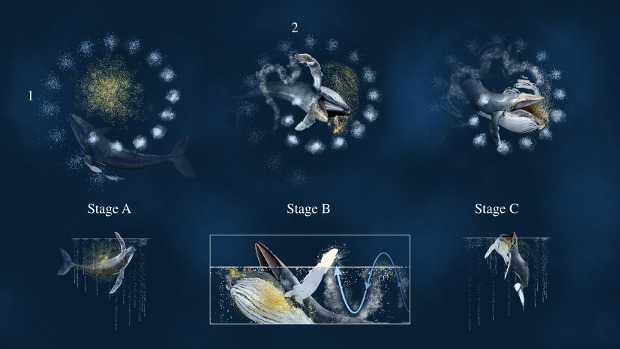
\includegraphics[width=\textwidth]{images/caza.jpg}
    \caption{Fases de la caza de la ballena jorobada}
    \end{figure}    
    \footnote{https://nmas1.org/news/2019/10/17/ballena-aletas-peces-boca}
    
\end{frame}
\begin{frame}{Ataque sobre la presa}
    
    Para modelas la fase de ataque sobre la presa usamos

    \begin{align}
        \begin{cases}
            X_i(t+1) &= e^{bl}cos(2\pi l)D_2 + X^* \\
            D^2_i &= ||X^*(t)-X_i(t)||\\
        \end{cases}\label{eq:2}
    \end{align}

\end{frame}
\begin{frame}{Resumen de los movimeintos}
    \[
    X_i(t+1) =  
\begin{cases}
    X^*(t) - A\cdot D^1_i & p < \frac{1}{2}\\
    e^{bl}cos(2\pi l)D^2_i + X^*  & p\geq \frac{1}{2}\\  
\end{cases}
    \]

\end{frame}
\begin{frame}{Pseudo-código de la metaheurística}
    \begin{figure}[H]
        \centering
        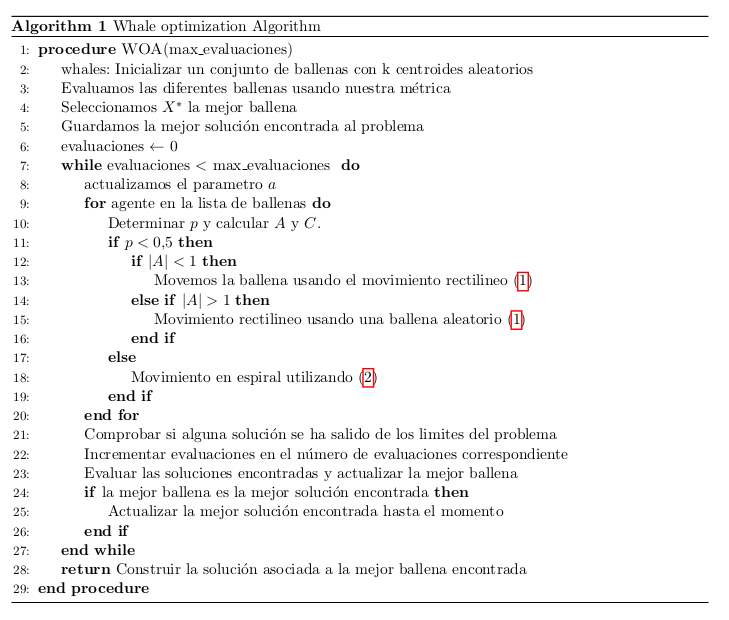
\includegraphics[width=0.9\textwidth]{images/code}
        \end{figure}    
\end{frame}
\end{document}